\documentclass[12pt,a4paper]{article}
\usepackage[english]{babel}
\usepackage[utf8]{inputenc}
\usepackage{amssymb,amsmath}
\usepackage[all]{xy}
\usepackage{url}
\usepackage{graphicx}
\usepackage{color}
\newcommand{\angstrom}{\textup{\AA}}
\color{black}
\usepackage{geometry}
\usepackage[autostyle]{csquotes}
\usepackage{tikz}
\usetikzlibrary{bayesnet}
\def\UrlBreaks{\do\/\do-}
\usepackage{dcolumn}
\usepackage{booktabs}
\usepackage{tikz}
\usetikzlibrary{positioning,shapes,arrows}
\newcolumntype{M}[1]{D{.}{.}{1.#1}}
\usepackage{upquote} % Upright quotes for verbatim code
\usepackage{fancyvrb} % verbatim replacement that allows latex
\usepackage{float}

\usepackage{amsmath}
\usepackage{algorithm}
\usepackage[noend]{algpseudocode}
\usepackage{listings}
\makeatletter
\def\BState{\State\hskip-\ALG@thistlm}
\makeatother

\geometry{
	a4paper,
 	left=15mm,
 	right=15mm,
 	top=10mm,
 	bottom=15mm
}

\DefineVerbatimEnvironment{Highlighting}{Verbatim}{commandchars=\\\{\}}

\newcommand{\VerbatimStringTok}[1]{\textcolor[rgb]{0.25,0.44,0.63}{{#1}}}



\begin{document}
\title{State-of-the-art Chinese Word Segmentation with Bi-LSTMs}
\author{Michał Ostyk-Narbutt (1854051)\\Prof. Roberto Navigli \\ Natural Language Processing Homework 1}

\maketitle


\begin{center}

\includegraphics[width=0.5\textwidth]{img/sapienza_logo.jpg}
\end{center}
\maketitle
%\tableofcontents
%\clearpage
\section{Introduction}
Chinese word segmentation (CWS) has gained a lot of popularity within the Natural Language Processing (NLP) community lately. This is especially the case since Deep Learning (DL) became prominent and Recurrent Neural Networks  (RNN) have been introduced.

In this project, we explore the use of Bi-directional Long Short Term Memory (LSTM) neural networks. This report will present the approach used, the architecture along with several hyperparameters and the end results. However, the biggest problem remains with dealing with Out-of-Vocabulary words (OOV).

\section{Dataset and State-of-the-Art}
In this project, we draw inspiration from \cite{paper}, where the researchers have built, and trained two Bi-LSTM's on 4 varying datasets ('as', 'msr', 'pku, 'cityu') each containing 'training' and 'validation' data which can be found here \cite{data}. These include two which were in Traditional Chinese which needed to be translated into simplified prior to training. The authors claim that their model outperforms most other state-of-the art models, reaching accuracy $\geq 95 \%$ on most datasets. 


Prior to training and building the model, the datasets underwent the following steps of preprocessing. First using HanziConv \cite{hanzi}, the Traditional datasets were converted to to Simplified Chinese. Then From the original file, two files were created; An Input File, which contains no spaces and serves as the X-data, as well as a Label File, which in BIES format serves as the target of classification (in reality these would be numerical classes). 

\section{Model and Approach}
The approach for building feature vectors from the dataset which would be fed to the model for training is explained in Algorithm \ref{euclid} below.

\begin{algorithm}
\caption{Model data creation}\label{euclid}
\begin{algorithmic}[1]
\item For each dataset, take the Input and label files for training and validation.

\item For the training Input file (no spaces):
\begin{algorithmic}[1]
\item create unigrams and bigrams for the entire text file
\item create separate vocabularies for unigrams and bigrams
\item while masking OOV create seperate dictionaries mapped by numbers.
\item read the Input file line by line and create feature vectors  (scalars) using the above dictionaries.
\end{algorithmic}

\item For the validation Input file (no spaces):
\begin{algorithmic}[1]
\item take the training dictionaries and create  feature vectors  (scalars) for each line of the text
\end{algorithmic}

\item For both Label files (no spaces):
\begin{algorithmic}[1]
\item Convert from BIES to numerical classes
\item perform one-hot-encoding.
\end{algorithmic}

\item for training purposes, pad accordingly for both files.

\end{algorithmic}
\end{algorithm}


In this paper, the utilised model is the non-stacking model from \cite{paper} shown on Figure \ref{img:model}. Initial testing proved that the stacking model gave much worse results. The last layer is of size 4 (number of BIES classes), and is activated using SoftMax. Several hyperparameters were explored, However, not using grid-search as it proved to be too expensive.
Some of the most effective ones are presented in Table \ref{table:hyper}.

\begin{table}[htb]
\centering
\caption{Hyperparameters of the BI-LSTM model}
\label{table:hyper}
\begin{tabular}{|l|l|l|l|l|}
\cline{1-2} \cline{4-5}
Embedding Layer $-$ Unigrams & 64     &  & Recurrent dropout & 0.35 \\ \cline{1-2} \cline{4-5} 
Embedding Layer $-$ Bigrams  & 16     &  & Batch size        & 128  \\ \cline{1-2} \cline{4-5} 
Learning rate                & 0.0015 &  & Hidden layer size & 256  \\ \cline{1-2} \cline{4-5} 
LSTM dropout                 & 0.4    &  & Padding size      & 30   \\ \cline{1-2} \cline{4-5} 
kernel regularizer l2        & 0.01   &  & bias regulizer l1 & 0.01 \\ \cline{1-2} \cline{4-5} 
\end{tabular}
\end{table}

\begin{figure}[H]

\begin{center}
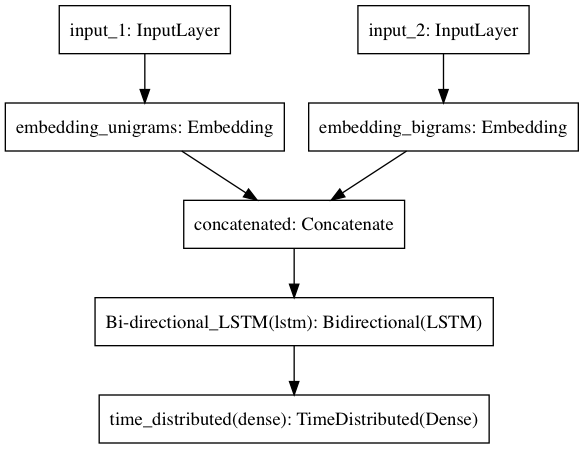
\includegraphics[width=0.7\columnwidth, angle = 0]{img/model.png}
\end{center}
\caption{Non-Stacking Model used for training, including two separate inputs for unigrams and bigrams.}
\label{img:model}
\end{figure}
\section{Results}
The best model was trained on the 'pku' and 'msr' datasets which amount 105980 samples for training and 5930 sample for validation.  Figure \ref{img:results} present the training results. As shown, the training stops quite early within 4 epochs. This is due to the imposed early stopping monitoring of the validation loss and precision.
As previously stated the padding size was set to 30. Other sizes were explored however, smaller proved to be to unstable, and larger was not representative of the data as the median line length far below 40.  For testing purposes the model has an extra None input layer which can intake variable line lengths, hence ideal for predictions of large files.
\begin{figure}[H]
\begin{center}
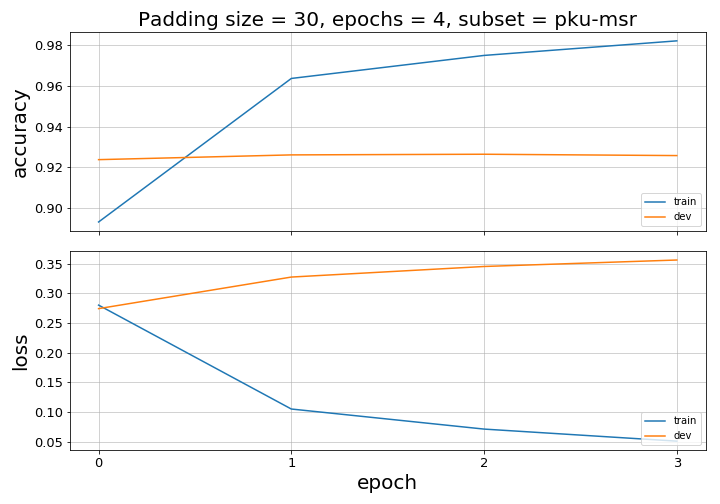
\includegraphics[width=0.7\columnwidth, angle = 0]{img/pku-msr.png}
\end{center}
\caption{Training and validation results compared using loss and accuracy}
\label{img:results}
\end{figure}
\section{Conclusion}


To sum up, the model achieves quite good accuracy, however, in this case we are more interested in precision which grows on slightly and then falls. Some of these flaws can be associated to OOV words, which could be slightly resolved better regularization and more data. The final validation (dev) accuracy seems promising but for the growing loss. 


\begin{thebibliography}{1}

\bibitem{paper} Ma, Ji \& Ganchev, Kuzman \& Weiss, David. (2018). State-of-the-art Chinese Word Segmentation with Bi-LSTMs. 
\bibitem{data} \url{http://sighan.cs.uchicago.edu/bakeoff2005/}
\bibitem{hanzi} \url{https://pypi.org/project/hanziconv/}

\end{thebibliography}

\end{document}
